\addcontentsline{toc}{chapter}{Appendices}
\appendix

\chapter{Interpretation of morphogen gradients by a bistable circuit}
\label{appendix:double-exclusive}
\includepdf[pages=1-51, offset=75 -90, scale=0.85, frame,
        clip,trim=20mm 5mm 20mm 15mm,
        pagecommand={}, addtotoc={
        2,section,1,Supplementary Figures,appendix:double-exclusive:figures,
        18,section,1,Supplementary Methods,appendix:double-exclusive:methods,
        19,subsection,2,Differential Equation Models \& Parameter Inference,appendix:double-exclusive:inference,
        40,subsection,2,Bistability Analysis,appendix:double-exclusive:bistability,
        42,subsection,2,Boundary Experiments,appendix:double-exclusive:boundaries,
        50,subsection,2,Models of the Exclusive Receiver Relay Circuits,appendix:double-exclusive:relay
}]{publications/double-exclusive-si.pdf}

\chapter{Parameter Inference with Bifurcation Diagrams}
\label{appendix:inference}
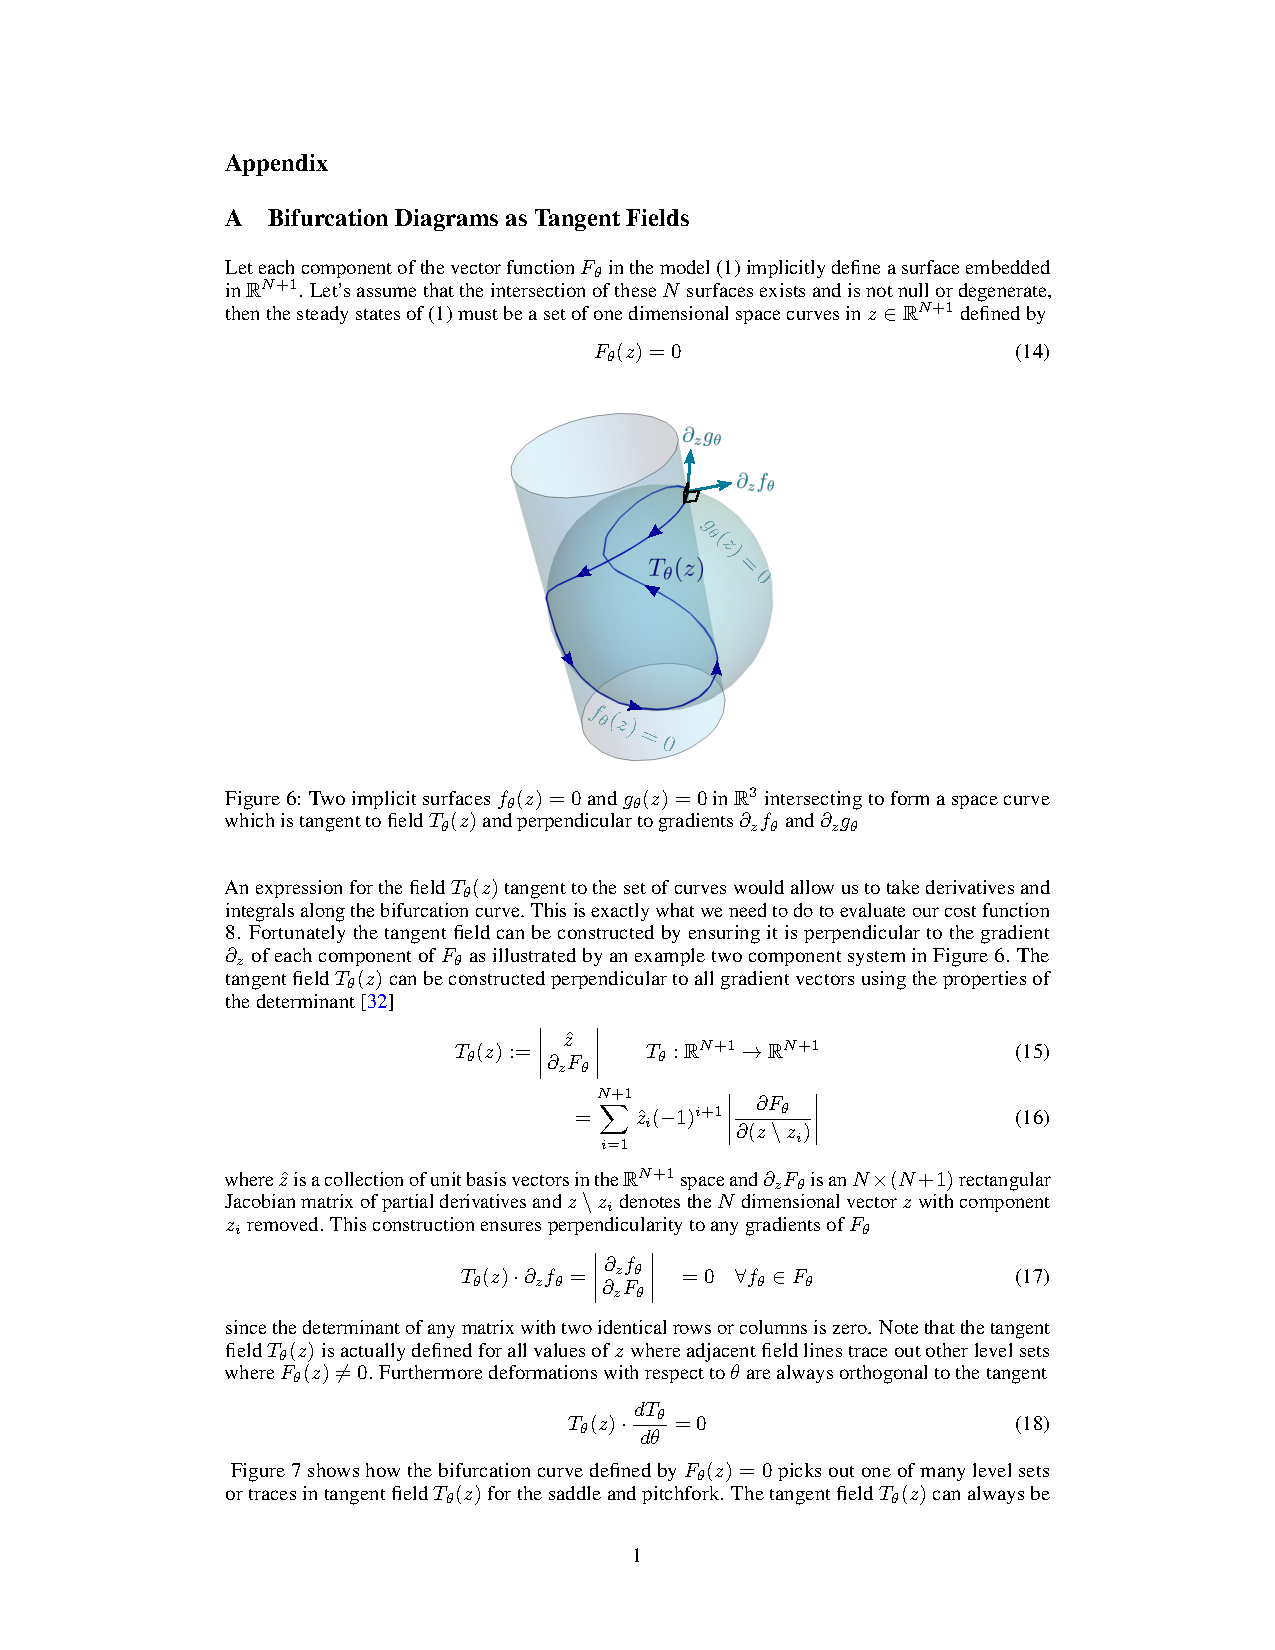
\includepdf[pages=1-4, offset=75 -90, scale=0.85, frame,
        clip,trim=25mm 5mm 25mm 15mm,
        pagecommand={}, addtotoc={
        1,section,1,Bifurcation Diagrams as Tangent Fields,appendix:tangent-fields,
        2,section,1,Conditions for Bifurcations,appendix:bifurcation-measure,
        3,section,1,Leibniz Rule for Space Curves,appendix:leibniz-rule
}]{publications/bifurcation-inference-si.pdf}
